% En esta sección se hace un breve mapeo documental de los avances 
% relacionados a la aplicación a desarrollar y es la base para demostrar 
% la validez del proyecto. Aquí se remarca que, aunque es un trabajo 
% profesional el mismo debe ser innovador y encontrarte en el estado del 
% arte de la ingeniería del software.

\noindent En la actualidad la mayoría de los videojuegos multijugador desarrollados
utilizan una arquitectura cliente-servidor, en la que el jugador
hace de cliente y se conecta a un servidor centralizado. Este servidor suele manejar
la mayor parte de la lógica del juego, como puede ser la simulación de las físicas, el procesamiento
de las acciones de los jugadores, la validación de las reglas del juego, entre otros.
Es común que algunas funcionalidades sean delegadas a otros servicios pero suelen ser funcionalidades
secundarias como el manejo de cuentas de usuario, guardado y consulta de estadísticas
o la gestión de partidas.

Dada la naturaleza monolítica que prevalece en este modelo de servidores centralizados, tenemos que la cantidad de eventos, y en consecuencia la cantidad de jugadores,
que un único servidor puede administrar se encuentra limitada por los recursos de hardware del mismo.
Esto resulta en una escalabilidad \textbf{vertical}, donde la única forma de aumentar la capacidad
de jugadores o eventos que un servidor puede manejar depende de la mejora de los recursos de hardware.

En un contexto tecnológico en el que la investigación y desarrollo de los procesadores
se encuentra en un punto de inflexión, donde la ley de Moore se encuentra en su límite,
donde se opta por incrementar la cantidad de núcleos ante la dificultad de aumentar la frecuencia de los mismos,
y donde cada vez más se prefiere los sistemas distribuidos como respuesta a las problemáticas surgientes,
es que decidimos explorar la posibilidad de desarrollar un videojuego multijugador
\textbf{altamente distribuido}.

% \noindent Akka es un toolkit desarrollado por la empresa Lightbend. Un toolkit es un conjunto de 
% bibliotecas compatibles entre sí, todas siendo parte de un mismo ecosistema. 
% Akka cuenta con APIs para Java y Scala, aunque puede ser utilizado con Kotlin también 
% gracias a su compatibilidad nativa con Java. Entre otras cosas, Akka provee:

% \begin{itemize}
%     \item Comportamiento multi-hilo nativo.
%     \item Transparencia para la comunicación de sistemas remotos.
%     \item Arquitectura elástica, clusterizada, altamente disponible y escalable a demanda.
% \end{itemize}

% Todo esto lo logra además haciendo uso del modelo de actores, un paradigma que simplifica 
% los sistemas concurrentes mediante la eliminación de la memoria compartida, reemplazando su uso 
% con el concepto de envío de mensajes. Este mecanismo evita muchos de los pitfalls que los paradigmas 
% concurrentes clásicos tienen (deadlocks, race conditions, etc) dado que cada actor sólo puede 
% actualizar su propio estado, compartiendo mediante mensajes a los demás actores los cambios de 
% estado del sistema.

% Godot es un motor para desarrollar videojuegos, argentino, gratuito y de código abierto. 
% Este motor permite crear tanto juegos 2D como también 3D. Además de ser multiplataforma, 
% permite programar scripts exponiendo una API orientada a objetos en los lenguajes C++, C\# 
% e incluso GDScript, un lenguaje propio de Godot.
% La filosofía de diseño de Godot es construir escenas reutilizables usando componentes básicos 
% llamados nodos. 
% A estas escenas y nodos se les puede agregar comportamiento con scripts. 
% Con la composición y jerarquía de los Nodos se puede construir una lógica de juego que es clara 
% y fácil de entender.


% \subsection{Arquitectura de juegos}
% \noindent Hoy en día, la arquitectura de la mayoría de los juegos en línea es la de un Cliente-Servidor clásico. 
% Mientras el juego y su lógica principal están corriendo en el Servidor, distintos jugadores (Clientes) 
% se conectan a él desde su máquina y, una vez conectados, comenzarán a enviar actualizaciones al 
% Servidor en base a las acciones del jugador. El Servidor recibe estas actualizaciones, 
% calcula las acciones que ocurrieron como resultados de ellas y computa el estado final de los 
% elementos del juego dentro de un game loop (el movimiento de un jugador, la interacción entre 
% personajes, el estado del/los niveles, etc.). Una vez computada la actualización del juego 
% responde a los Clientes conectados con el nuevo estado, para que los mismos puedan actualizar 
% su estado local. De esta forma los clientes mantienen sincronizado el estado del juego localmente 
% y renderizan en base al mismo.

% \begin{figure}[htbp]
%     \centering
%     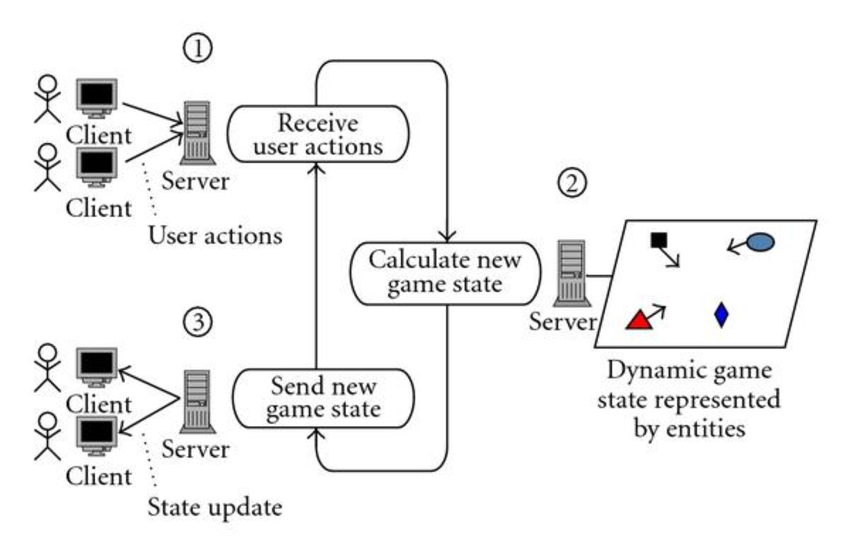
\includegraphics[width=0.5\textwidth]{../assets/monolith-server-game-loop.png}
%     \caption{Diagrama de flujo del game loop de los servidores monolíticos clásicos}
% \end{figure}
